\documentclass[12font]{article}
\title{\textbf{Non-Simply Connected Subsystems and the Reduced Density Matrices}}
\author{Chen-Chih Wang  }
\date{\textit{Department of Physics, National Tsing Hua University, Hsinchu 30013, Taiwan} \\ (Dated: \today)}
\usepackage[margin=2cm]{geometry}
%\usepackage[fleqn]{amsmath}
%\usepackage{CJK,amsmath}
\usepackage{amsfonts,amssymb}
\usepackage{amsmath}
\numberwithin{equation}{section}    % numbering equations by their section
\usepackage{fancyhdr}
%\pagestyle{fancy}
\usepackage{textcomp}
\usepackage{graphicx}
\usepackage{float}
\usepackage{color}
\usepackage{tikz}
\usepackage{multicol}
\usepackage{threeparttable}
\usepackage{amsthm}
\usepackage{mathtools}
\usepackage{hyperref}
\urlstyle{same}
\usepackage{caption}
\usepackage{subcaption}
\usepackage{dsfont}
\usepackage{qcircuit} % quantum circuit

\usepackage{mathrsfs} % for \mathscr

\usepackage{algorithm}
\usepackage{algpseudocode}

% \usepackage{tensor-network}
% \tnsetup{tensorsize=16pt, xscale=0.9, yscale=0.6, outer ysep=7pt}

\newtheorem{theorem}{Theorem}[section]
\theoremstyle{definition}
\newtheorem{definition}{Definition}[section]
\newtheorem{lemma}[theorem]{Lemma}
\newtheorem{corollary}{Corollary}[theorem]
\newtheorem{proposition}[theorem]{Proposition}

\hypersetup{
    colorlinks=true,
    linkcolor=blue,
    filecolor=magenta,      
    urlcolor=blue,
    pdftitle={Overleaf Example},
    pdfpagemode=FullScreen,
    }
\usepackage[numbers,sort&compress]{natbib}

\newcommand{\vac}{\mrm{vac}}
\newcommand{\Bra}[1]{\left\langle #1 \right|}
\newcommand{\Ket}[1]{\left| #1 \right\rangle}
\newcommand{\bra}[1]{\langle #1 |}
\newcommand{\ket}[1]{| #1 \rangle}
\newcommand{\anglelr}[1]{\langle #1 \rangle}
\newcommand{\Anglelr}[1]{\left\langle #1 \right\rangle}
\newcommand{\braket}[2]{\langle #1 | #2 \rangle}
\newcommand{\Bbraket}[2]{\left\langle #1 \right|\left. #2 \right\rangle}
\newcommand{\dif}[1]{\frac{\mathrm{d}}{\mathrm{d}#1}}
\newcommand{\diff}[2]{\frac{\mathrm{d}#1}{\mathrm{d}#2}}
\newcommand{\gd}{\boldsymbol{\nabla}}
\newcommand{\dive}{\boldsymbol{\nabla}\cdot}
\newcommand{\curl}{\boldsymbol{\nabla}\times}
\newcommand{\lrno}[1]{\left.#1\right.}
\newcommand{\lr}[1]{\left(  #1  \right)}
\newcommand{\lrm}[1]{\left[  #1  \right]}
\newcommand{\lrg}[1]{\left\{  #1  \right\}}
\newcommand{\lri}[1]{\left. #1 \right.}  % invisible bracket
\newcommand{\abs}[1]{\left|  #1  \right|}
\newcommand{\de}{\partial}
\newcommand{\pdif}[1]{\frac{\partial}{\partial#1}}
\newcommand{\pdiff}[2]{\frac{\partial#1}{\partial#2}}
\newcommand{\mrm}[1]{\mathrm{#1}}
\newcommand{\bo}[1]{\mathbf{#1}}
\newcommand{\bog}[1]{\boldsymbol{#1}}
\newcommand{\vint}[3]{\int_{#1}#2\cdot\mathrm{d}\mathbf{#3}}
\newcommand{\voint}[3]{\oint_{#1}#2\cdot\mathrm{d}\mathbf{#3}}
\newcommand{\Vint}{\int\mrm{d}^3\bo{r}'}
\newcommand{\rr}{\mathbf{r} - \mathbf{r}'}
\newcommand{\arr}{\left|\mathbf{r} - \mathbf{r}'\right|}
\newcommand{\nx}{\hat{\bo{n}}_1}
\newcommand{\ny}{\hat{\bo{n}}_2}
\newcommand{\alert}[1]{{\color{red}#1}}
\newcommand{\alertV}[1]{{\color{violet}#1}}
\newcommand{\Tr}{\mrm{Tr}}
\newcommand{\tTr}{\mrm{tTr}}
\newcommand{\tr}{\mrm{tr}}
\newcommand{\norm}[1]{\left\lVert#1\right\rVert}
\newcommand{\tcor}[2]{\langle -ic_{#1}c_{#2} \rangle_M}

\newcommand{\wordfig}[2]{\begin{minipage}[h]{#1 cm}
	\vspace{0pt}
	\includegraphics[width=\textwidth]{#2}
   \end{minipage}}
   
% \newcommand{\cnot}{\mrm{CNOT}}

% \newcommand{\arrequ}[1]{\begin{aligned}#1\end{aligned}}

% \newcommand{\Qcirc}[1]{\begin{minipage}[h]{0.7cm}
% 	\vspace{0pt}
% 	\Qcircuit @C=1em @R=.7em {#1}
%    \end{minipage}}
\newcommand{\dimer}[2]{\sigma_{#1}^{\alpha_{#1#2}}\sigma_{#2}^{\alpha_{#1#2}}}

\begin{document}
\maketitle
\renewcommand\qedsymbol{$\blacksquare$}



\fontsize{12pt}{16pt}\selectfont

\begin{abstract}
    The reduced density matrix of a multiply connected subsystem exhibits an exact diagonal structure different from that of a simply connected subsystem. 
\end{abstract}

% \tableofcontents
First, we consider a non-simply connected region $A$ with an interior hole. The reduced density matrix of this subsystem is as follows,
\[
    \rho_{A}
    =
    \frac{1}{2^{N^A - N^A_p}}
    \hat{\Pi}_A
    \lr{\mathds{1} + W_\mathcal{L}}
    \sum_{[\mathfrak{D}]\subset A}
    \lr{
        \mathfrak{C}_\mathfrak{D} \Sigma_\mathfrak{D} 
        +
        \mathfrak{C}_{\mathfrak{D} \ominus \mathfrak{H}} \Sigma_{\mathfrak{D}\ominus\mathfrak{H}}
    }
\]
where $\mathcal{L}$ is a closed loop inside the subsystem $A$ that encloses the hole. In other words, the loop $\mathcal{L}$ is a non-contractible loop according to the non-simply connected subsystem $A$. The edge configuration $\mathfrak{H}$ represents the \textit{web-patch} configuration of the hole enclosed by $A$ consisting of all the dimers inside the hole and those that cross the inner boundary.
\[
    \rho_A
    =
    \frac{1}{2^{N^A - N^A_p - 1}}
    \hat{\Pi}_A
    \lr{
    \frac{\mathds{1} + W_\mathcal{L}}{2}
    }
    \sum_{[\mathfrak{D}]\subset A}
    \lr{
        \mathds{1} 
        + 
        \underbrace{
            \varphi(\mathfrak{H},\mathfrak{D}) \frac{\mathfrak{C}_{\mathfrak{D}\ominus\mathfrak{H}}}{\mathfrak{C}_\mathfrak{D}}
        }_{\equiv 2p_\mathfrak{D}-1 }
        \Sigma_\mathfrak{H}
    }
    \mathfrak{C}_\mathfrak{D}
    \Sigma_\mathfrak{D} 
\]

\[
    \rho_A
    =
    \frac{1}{2^{N^A - N^A_p - 2}}
    \hat{\Pi}_A
    \hat{\Pi}_\mathcal{L}
    \sum_{[\mathfrak{D}]\subset A}
    \lrm{
        p_\mathfrak{D}
        \lr{
        \frac{\mathds{1} + \Sigma_\mathfrak{H}}{2}
        }
        +
        (1 - p_\mathfrak{D})
        \lr{
        \frac{\mathds{1} - \Sigma_\mathfrak{H}}{2}
        }
    }
    \mathfrak{C}_\mathfrak{D}
    \Sigma_\mathfrak{D} 
\]

\[
    \rho_A
    \equiv
    \frac{1}{2^{N^A - N^A_p - 2}}
    \hat{\Pi}_A
    \hat{\Pi}_\mathcal{L}
    \lrm{
        \lr{
        \hat{\Pi}_\mathfrak{H}^{(+)}
        \sum_{[\mathfrak{D}]\subset A}
        \tilde{\mathfrak{C}}^{(+)}_\mathfrak{D} \Sigma_\mathfrak{D}
        }
        \oplus
        \lr{
        \hat{\Pi}_\mathfrak{H}^{(-)}
        \sum_{[\mathfrak{D}]\subset A}
        \tilde{\mathfrak{C}}^{(-)}_\mathfrak{D} \Sigma_\mathfrak{D}
        }
    }
\]

\[
p_\mathfrak{D}
=
\frac{1}{2}
\lr{
        1
        + 
        \varphi(\mathfrak{H},\mathfrak{D}) \frac{\mathfrak{C}_{\mathfrak{D}\ominus\mathfrak{H}}}{\mathfrak{C}_\mathfrak{D}}
    }
\]

\[
\left\{
\begin{aligned}
    & \tilde{\mathfrak{C}}_\varnothing^{(+)} = p_\varnothing = \frac{1 + \mathfrak{C}_\mathfrak{H}}{2} \\
    & \tilde{\mathfrak{C}}_\varnothing^{(-)} = 1 - p_\varnothing = \frac{1 - \mathfrak{C}_\mathfrak{H}}{2}
\end{aligned}
\right.
\]

\[
\hat{\Pi}^{(\pm)}_\mathfrak{H}
=
\frac{\mathds{1} \pm \Sigma_\mathfrak{H}}{2}
\]

\[
\Tr_A\lr{\hat{\Pi}_A \hat{\Pi}_\mathcal{L} \hat{\Pi}_\mathfrak{H}^{(\pm)}} = 2^{N^A - N^A_p - 2}
\]

\begin{figure}
    \centering
    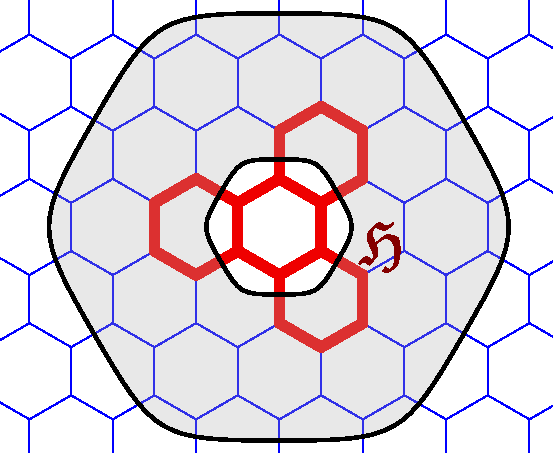
\includegraphics[width=0.4\linewidth]{figures/web-patch.pdf}
    \caption{The web-patch configuration $\mathfrak{H}$ covering the interior hole of a non-simply connected subsystem. Its corresponding string operator $\Sigma_\mathfrak{H}$ commutes with other string operators lying within the shaded subsystem.}
    \label{fig:web-patch-config}
\end{figure}

\[
\lr{\wordfig{3}{figures/web-patch.pdf}}
=
\lr{\wordfig{3}{figures/gauge-link.pdf}}
\ominus
\lr{\wordfig{3}{figures/raw-web.pdf}}
\]


\begin{equation}
    \rho_A
    =
    \frac{1}{2^{N^A - N^A_p - 2g}}
    \hat{\Pi}_A
    \hat{\Pi}_g
    \bigoplus_{\lrg{s}}
    \lrm{
        \hat{\Pi}_\mathfrak{H}^{(\lrg{s})}
        \sum_{[\mathfrak{D}]\subset A}
        \tilde{\mathfrak{C}}^{(\lrg{s})}_\mathfrak{D} \Sigma_\mathfrak{D}
    }
\end{equation}
\begin{equation}
    \left\{
    \begin{aligned}
        &\hat{\Pi}_g \equiv
        \prod_{n=1}^{g}\lr{\frac{\mathds{1} + W_{\mathcal{L}^{(n)}}}{2}} \\
        &\hat{\Pi}_\mathfrak{H}^{(\lrg{s})} \equiv 
        \prod_{n=1}^{g}\lr{\frac{\mathds{1} + s_n\Sigma_{\mathfrak{H}^{(n)}}}{2}} 
    \end{aligned}
    \right.
\end{equation}

\bibliographystyle{my_apsrev4-2}
% \bibliography{ref}% Produces the bibliography via BibTeX.




\end{document} 